\section{Pipes }\label{pipes}

\subsection{Heat Transfer Pipes (Objects: Pipe:Indoor \& Pipe:Outdoor)}\label{heat-transfer-pipes-objects-pipeindoor-pipeoutdoor}

\subsubsection{Heat Loss and Time Delay in Pipes}\label{heat-loss-and-time-delay-in-pipes}

The effects of heat loss and time delay in plant loop pipes exposed to air (Pipe:Indoor and Pipe:Outdoor) can be modeled explicitly in EnergyPlus. Users can select the environment with which the pipe transfers heat. Currently users have three options: `OutdoorAir', `Zone' and `Schedule'. Simulation for each of the environments is similar except the way in which the heat transfer between the pipe outer wall and the surrounding environment is calculated. When using the `OutdoorAir' option, the current outdoor dry-bulb temperature and wind velocity from the weather file (or design day input) are used. When the environment is specified as `Zone', the mean air temperature and room air velocity of the corresponding zone are used.

In the case of a pipe in a zone, the heat loss or gain is accounted for in the pipe heat transfer calculation and is also included in the zone air heat balance calculations. When the environment is specified as `Schedule', the user specifies a temperature and velocity schedule which will be used to calculate the heat transfer.

Pipe heat transfer in EnergyPlus is simulated by discretizing the pipe length into a number of nodes (20) and is an implementation of the model by Hanby et al. (2002). A control volume drawn around a node in the pipe is shown in Figure~\ref{fig:control-volume-drawn-around-node-i}. Three nodes are defined at each discrete section of the pipe and represent the fluid, pipe wall and external environment. The fluid and pipe have defined thermal capacitance (mass). The insulation around the pipe is currently modeled as steady-state (no thermal mass), and so the effect of this resistance is accounted for within the h\(_{f}\) term in the following description.~ For the fluid, there is one-dimensional flow from each upstream node.

\begin{figure}[hbtp] % fig 261
\centering

\includegraphics[width=0.9\textwidth, height=0.9\textheight, keepaspectratio=true]{media/image5831.png}
\caption{Control Volume drawn around node *i* \protect \label{fig:control-volume-drawn-around-node-i}}
\end{figure}

The model is formulated from the heat balances on the fluid and wall nodes.

\begin{equation}
{M_{f,i}}{C_{P,f}}\frac{{d{T_{f,i}}}}{{dt}} = \dot m{C_{P,f}}\left( {{T_{f,i - 1}} - {T_{f,i}}} \right) - {h_f}{A_i}\left( {{T_{f,i}} - {T_{w,i}}} \right)
\end{equation}

\begin{equation}
{M_{w,i}}{C_{P,w}}\frac{{d{T_{w,i}}}}{{dt}} = {h_f}{A_i}\left( {{T_{f,i}} - {T_{w,i}}} \right) - {h_e}{A_i}\left( {{T_{w,i}} - {T_e}} \right)
\end{equation}

where subscripts \emph{w}, \emph{f} and \emph{e} denote the values for pipe wall, fluid and environment, respectively. The current node is represented by a subscript of \emph{i}, while the previous node is represented by \emph{i-1}.  In the previous two equations, the terms are defined by:

\(M\) is the mass

\({C_p}\) is the specific heat

\(\dot m\) is the mass flow rate of fluid in pipe

\(T\) is the Temperature

\(A\) is the heat transfer area

\(h\) is the film convective resistance

\(t\) is time.

The exterior film convective resistance is calculated based on either wind speed, room air velocity, or a scheduled value based on the type of pipe heat transfer object. However, when the velocity gets too low, natural convection must be modeled. This is handled within the program by having a lower limit on the Nusselt number. For natural convection from a horizontal cylinder, a constant Nusselt number is assumed based on information from Spang (referenced below). This Nusselt number is 0.36. The Nusselt number used in calculating the exterior convection coefficient (Incropera and Dewitt 1996) is the maximum of the Nusselt number from the forced convection coefficient correlation and this natural convection Nusselt number (0.36).

In addition, the exterior resistance from the pipe wall inner surface to the environment will include resistance values for the pipe wall itself and any insulation specified around the pipe. This is treated as steady state value, so the simulation results are not affected by a change in insulation specific heat. However, the resistance is calculated based on thermal conductivity and thickness (using radial coordinate system), so the simulation results will vary with material conductivity changes. Again, this resistance is added in series with the exterior surface film convective resistance such that h\(_{f}\) contains film and insulation resistance.

Approximating the derivatives using backward differencing enables these equations to be represented as simultaneous algebraic equations. For the fluid, at time step n, the heat balance is:

\begin{equation}
\frac{{{M_{f,i}}{C_{P,f}}}}{{\Delta t}}\left( {T_{f,i}^n - T_{f,i}^{n - 1}} \right) = \dot m{C_{P,f}}\left( {T_{f,i - 1}^n - T_{f,i}^n} \right) - {h_f}{A_i}\left( {T_{f,i}^n - T_{w,i}^n} \right)
\end{equation}

Rearranging gives:

\begin{equation}
T_{f,i}^n\left[ {{M_{f,i}}{C_{P,f}} + \dot m{C_{P,f}}\Delta t + {h_f}{A_i}\Delta t} \right] = \dot m{C_{P,f}}\Delta tT_{f,i - 1}^n + {h_f}{A_i}\Delta tT_{w,i}^n + {M_{f,i}}{C_{P,f}}T_{f,i}^{n - 1}
\end{equation}

or:

\begin{equation}
{a_1}T_{f,i}^n = {a_2}T_{f,i - 1}^n + {a_3}T_{w,i}^n + {a_4}T_{f,i}^{n - 1}
\label{eq:PipeEquation614}
\end{equation}

where:

\begin{equation}
  \begin{array}{rl}
    a_1 &= M_{f,i}C_{p,f} + \dot{m}C_{p,f} \Delta t + h_f A_i \Delta t \\
    a_2 &= \dot{m} C_{p,f} \Delta t \\ 
    a_3 &= h_f A_i \Delta t \\
    a_4 &= M_{f,i} C_{p,f}
  \end{array}
\end{equation}

Similarly, taking backwards differences for the conduit wall at time step n, the heat balance becomes:

\begin{equation}
\frac{{{M_{w,i}}{C_{P,w}}}}{{\Delta t}}\left( {T_{w,i}^n - T_{w,i}^{n - 1}} \right) = {h_f}{A_i}\left( {T_{f,i}^n - T_{w,i}^n} \right) - {h_e}{A_i}\left( {T_{w,i}^n - T_e^n} \right)
\end{equation}

Rearranging gives:

\begin{equation}
T_{w,i}^n\left[ {{M_{w,i}}{C_{P,w}} + {h_f}{A_i}\Delta t + {h_e}{A_i}\Delta t} \right] = {h_f}{A_i}\Delta tT_{f,i}^n + {h_e}{A_i}\Delta tT_e^n + {M_{w,i}}{C_{P,w}}T_{w,i}^{n - 1}
\end{equation}

or:

\begin{equation}
{b_1}T_{w,i}^n = {b_2}T_{f,i}^n + {b_3}T_{e,i}^n + {b_4}T_{w,i}^{n - 1}
\label{eq:PipeEquation617}
\end{equation}

where:

\begin{equation}
  \begin{array}{rl}
    b_1 &= M_{w,i} C_{p,w} + h_f A_i \Delta t + h_e A_i \Delta t \\
    b_2 &= h_f A_i \Delta t \\
    b_3 &= h_e A_o \Delta t \\
    b_4 &= M_{w,i} C_{p,w}
  \end{array}
\end{equation}

Substituting Equation~\ref{eq:PipeEquation617} into Equation~\ref{eq:PipeEquation614} gives an equation for the current fluid temperature:

\begin{equation}
{a_1}T_{f,i}^n = {a_2}T_{f,i - 1}^n + {a_3}\left( {{b_2}T_{f,i}^n + {b_3}T_{e,i}^n + {b_4}T_{w,i}^{n - 1}} \right)/{b_1} + {a_4}T_{f,i}^{n - 1}
\end{equation}

\begin{equation}
T_{f,i}^n = \frac{1}{{\left( {{a_1} - {a_3}{b_2}/{b_1}} \right)}}\left[ {{a_2}T_{f,i - 1}^n + {a_3}\left( {{b_3}T_{e,i}^n + {b_4}T_{w,i}^{n - 1}} \right)/{b_1} + {a_4}T_{f,i}^{n - 1}} \right]
\label{eq:PipeTfitothen}
\end{equation}

The conduit is simulated by solving Equation~\ref{eq:PipeTfitothen} followed by Equation~\ref{eq:PipeEquation614} for each of the twenty cells in the model and incrementing the time step. The fluid temperature of the last node is taken to be the pipe outlet temperature.

\subsubsection{References}\label{references-036}

Hanby, V.I., Wright, J.A., Fletcher, D.W and Jones, D.N.T. 2002. Modeling the Dynamic Response of Conduits. International Journal of HVACR\&R, Vol.8, No.1. pp.~1-12.

Incropera, F.P. and Dewitt, D.P. 1996. Fundamentals of Heat Transfer, 4th Edition, pp.~369-370.

Spang, Bernhard. Correlations for Convective Heat Transfer. Chemical Engineers' Resource Page:

\subsection{Underground Pipe (Object: Pipe:Underground)}\label{underground-pipe-object-pipeunderground}

\subsubsection{Description of Model}\label{description-of-model-000}

The buried pipe model in EnergyPlus is similar to the other pipe heat transfer objects (i.e., Pipe:Indoor and Pipe:Outdoor) except for the way in which the pipe boundary condition is developed. For a buried pipe the ground between the pipe and the surface must be modeled. For a shallow buried pipe, the GroundHeatExchanger:Surface object may be used, which uses modified conduction transfer functions to model the ground. However, beyond a certain thickness, the transfer function method fails, and EnergyPlus will respond with a fatal error due to convergence problems. Therefore, when a pipe is buried deeper than about one meter, this new buried pipe model should be used. When the pipe is buried shallower than one meter, either model may be used. Due to the finite difference nature of the Pipe:Underground model, the GroundHeatExchanger:Surface may be slightly faster and therefore more desirable.

The buried model develops a grid around the pipe. The grid was based originally on a model by Piechowski (1999), and still carries the model nomenclature. The grid extends from the ground surface down to a calculated distance below the pipe. The domain extends sideways from the symmetric center of the pipe to a calculated distance from the pipe. The grid stretches along the full length of the pipe. At each cross section, transient 2D Cartesian finite difference equations are used, updating each node except the node centered on the pipe. Axial heat transfer is not modeled in the soil. The large view of the outer Cartesian grid system is shown in Figure~\ref{fig:pipe-underground-outer-finite-difference-grid}.

\begin{figure}[hbtp] % fig 262
\centering

\includegraphics[width=0.9\textwidth, height=0.9\textheight, keepaspectratio=true]{media/image5851.png}
\caption{Pipe:Underground Outer Finite Difference Grid \protect \label{fig:pipe-underground-outer-finite-difference-grid}}
\end{figure}

When the model encounters the pipe node, the existing model for Pipe:Interior and Pipe:Exterior pipes is used. The finite difference temperatures neighboring the pipe, grid spacing and soil properties are used to create an average boundary temperature for the pipe along with a conductance value. With a boundary temperature available and a conductance value mimicking the convection coefficient, the simulation continues exactly as with the other pipe heat transfer objects. To avoid redundancy, see the Pipe:Indoor or Pipe:Outdoor objects for a detailed description of the pipe model.

\subsubsection{Boundary Conditions}\label{boundary-conditions-000}

The boundary conditions for this model include a symmetric vertical boundary centered on the pipe, the ground surface, a `far-field', and a `deep ground'. The ground surface boundary uses current simulation outdoor dry-bulb temperature, and the user-entered convection coefficient. The `far-field' and `deep ground' temperatures come from the ``undisturbed'' ground temperature object specified in the input.

Currently, the model is set up to be exposed to open soil above the pipe. If the user intends on simulating this buried pipe under a foundation slab, the effects can be approximating by use of the basement/slab heat transfer preprocessor program. This program takes in general building information, and performs a simulation which generates ground temperatures. Typically these effects are used to generate boundary conditions for the floor zone, but they may also be used in generating the ground surface temperatures for this pipe model. The data from the slab program will be monthly temperatures, so the user can use these as a surface ground temperature object which provides boundary data to the Pipe:Underground model.

\subsubsection{Geometry}\label{geometry}

The model develops the pipe depth and ground thickness from the user-entered construction information. The soil, pipe wall, and optional pipe insulation are entered as materials (with inherent thicknesses). The soil is entered as a standalone material, while the pipe insulation (if applicable) and the pipe wall should be given as a construction containing one or two materials. With knowledge of each individual thickness, the pipe geometry is obtained. The pipe length and inside diameter are the only additional geometry inputs.

\subsubsection{Model Assumptions}\label{model-assumptions-000}

\begin{itemize}
\item
  Constant properties throughout domain
\item
  Moisture is not directly involved with the model operation, so careful selection of soil thermal conductivity is a priority
\item
  Negligible axial heat transfer compared to radial heat transfer
\item
  Axisymmetric heat transfer in near pipe region
\item
  Surface convection coefficient is constant throughout simulation (does not vary with wind speed)
\end{itemize}

\subsubsection{References}\label{references-1-015}

Kusuda, T. \& Achenbach, P. 1965. `Earth Temperature and Thermal Diffusivity at Selected Stations in the United States', ASHRAE Transactions Vol. 71, Part 1, pp.~61--75.

Piechowski, M. 1999. `Heat and Mass Transfer Model of a Ground Heat Exchanger: Theoretical Development', Energy Research 23 (7), pp.~571--588.

\subsection{PipingSystem:Underground Simulation}\label{pipingsystemunderground-simulation}

In order to simulate diverse underground piping systems, a generalized model has been implemented which allows placement of pipes in a solid medium (soil).~ The model simulates circuiting effects of multiple pipes by allowing fluid to flow in the pipes in different directions.~ The model also has the capability of simulating interaction with zone surfaces to account for things such as basement heat transfer in a foundation heat exchanger.~ Different aspects of the modelling approach are described in this section which can assist the user in determining if this model is appropriate for a particular application, and determining input parameter values.

An alternative interface is implemented which provides a simpler set of inputs for simulating horizontal trench heat exchangers.~ The key limitations of the simpler inputs include all piping in the domain being on a single circuit, all trenches equidistance apart, and each trench with the same burial depth.~ If this is satisfactory for an application, the GroundHeatExchanger:HorizontalTrench object is a suitable object.~ The object uses the same underlying simulation algorithms and data structures as the detailed piping system model, but with a simpler set of input parameters.~ For other cases and more detailed studies, the PipingSystem:Underground:* objects provide full flexibility.

A dual-coordinate system finite volume heat transfer model of pipes buried in a conducting medium is employed.~ The dual-coordinate system consists of a coarse Cartesian system in the conducting region (the soil, for example) with a refined radial system in the near-pipe region.~ The pipes are connected as objects on the plant loop and are simulated as needed during loop convergence, while the ground itself is only simulated once per system time step.

\subsubsection{Approach:}\label{approach-002}

\subsubsection{General Development and Solution Scheme}\label{general-development-and-solution-scheme}

A new heat transfer model is implemented to handle a diverse set of buried pipe conditions.~ The model uses a dual-coordinate system approach to solve a finite volume domain in a computationally efficient manner.~ The main idea behind the dual coordinate system technique is to focus the computational effort to the region where it is most needed: near the pipe(s).~ To this end, a coarse grid Cartesian coordinate system is used to solve the slow-moving ground heat transfer.~ Then, within one of these cells, a radial coordinate system is configured around the pipe/insulation with a specialized interface cell between the systems.~ Figure~\ref{fig:radial-near-pipe-cell-within-a-cartesian-cell} shows an example of cells surrounding a pipe, including the radial region in the near-pipe cell, while Figure~\ref{fig:close-up-view-of-example-radial-cell} shows a zoomed-in view of the near-pipe cell itself.

\begin{figure}[hbtp] % fig 263
\centering
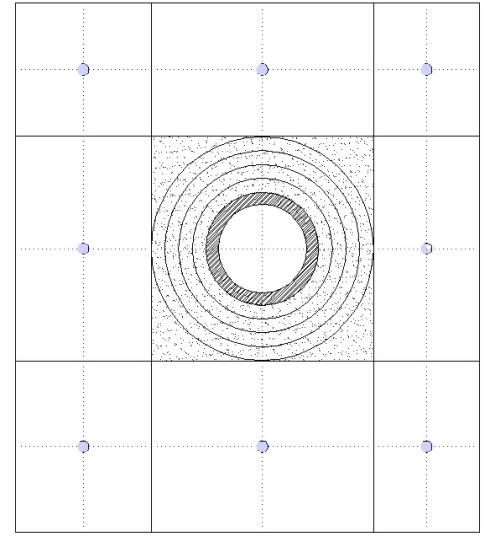
\includegraphics[width=0.9\textwidth, height=0.9\textheight, keepaspectratio=true]{media/image5852.png}
\caption{Radial "near-pipe" cell within a Cartesian cell \protect \label{fig:radial-near-pipe-cell-within-a-cartesian-cell}}
\end{figure}

\begin{figure}[hbtp] % fig 264
\centering
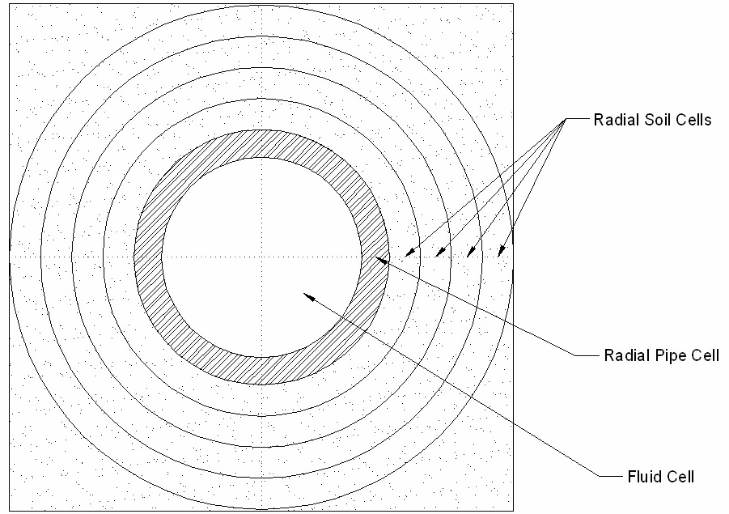
\includegraphics[width=0.9\textwidth, height=0.9\textheight, keepaspectratio=true]{media/image5853.png}
\caption{Close-up view of example radial cell \protect \label{fig:close-up-view-of-example-radial-cell}}
\end{figure}

The ground heat transfer model can be set up in a fully-3D or quasi-3D manner.~ In either case, there is a three-dimensional grid of Cartesian cells placed in the domain.~ In fully-3D mode, the axial heat transfer is accounted for; in quasi-3D mode, the axial effects are ignored and the result is essentially a set of 2D slices along the length of the domain.~ The determination of which method will be utilized in the final model shall be based upon final testing and on a balance between accuracy vs.~computation time.~ This option could be left to the end-user, but this will likely be unnecessary input overhead.

A fully implicit (and thus numerically stable) formulation is used to describe all cells, which means an iteration loop must be implemented.~ In this solver, an outer iteration loop is used to bring the entire domain to convergence, while an inner iteration loop is used over all the radial cells.~ This is intended to focus the computational effort even further.~ The outer region may converge within one or two iterations, while the ``near-pipe'' cells may take much more iteration.~ For this reason, it does not make sense to iterate over the entire domain a large number of times.

\subsubsection{Boundary Conditions}\label{boundary-conditions-1}

The farfield boundary condition is defined by a Kusuda and Achenbach (1965) correlation, which requires annual ground surface temperature data.~ As with the current Pipe:Underground model, the user will be able to enter the correlation parameters directly, or information from the monthly ground temperature input object will be used to infer the parameters.

The ground surface boundary condition is defined by an energy balance between the surrounding interior cells and the ground surface, including convection and radiation.~ As with the Pipe:Underground object, the ground surface sun exposure may be an optional input to allow for a shaded ground surface.~ In addition to the standard conduction, convection, and both short- and long-wave solar radiation at the surface, the ground surface boundary condition also includes the effects of evapotranspiration in the surface vegetation---the heat loss due to evaporation from soil to plant surface, and transpiration internal to the plant itself.~ The evapotranspiration rate is calculated as a moisture loss by using the Walter et al. (2005) model, and translated into a heat loss by multiplication with the density and latent heat of evaporation of water.~ The evapotranspiration rate is dependent on the type of vegetation at the surface; the user can vary the surface vegetation from anywhere between a concrete surface and a fairly tall grass (about 7'').

Based on the application, an adiabatic boundary condition will also be implemented and employed on particular surfaces of the domain.~ For the case where a basement or under-slab region is present, for example, an adiabatic boundary will represent the vertical line of symmetry.

\subsubsection{``Pipe Cell'' Simulation}\label{pipe-cell-simulation}

The ground is discretized into coarse Cartesian cells, some of which will contain a pipe.~ These ``pipe-cells'' are further discretized into a radial system with a specialized interface cell to couple these systems.~ The radial cells consist of a number of ground cells, with an optional insulation cell, then the pipe cell, followed by the fluid itself.

The fluid is modeled as a cylindrical cell interacting with incoming fluid and heat transfer to the pipe.~ When there is no flow in the system, the cell essentially becomes radially adiabatic so that the fluid temperature will float during off periods.~ It will not be equal to ground temperatures, unless it is off for a long time and the transient heat is allowed to dissipate.~ When there is flow in the system, the incoming fluid and heat transfer from the pipe wall balance with the mass of the cell to come up with a new fluid temperature for that cell, to be passed downstream to the next cell.

The fluid within the cells is modeled directionally, so that the flow can be circuited through multiple pipe segments in different directions.~ The flow direction in each pipe is specified by a choice field input.

\subsubsection{Basement Interaction}\label{basement-interaction}

The model can also interact with basement surfaces.~ The interaction is split into two sections: floor surfaces and wall surfaces.~ For each of these, the analysis is lumped, i.e., all walls are treated as one average wall surface and all floors are treated as one average floor surface.~ The distance that the basement impinges within the domain is defined by a simple width and height specification.~ The domain is then \emph{cutaway} for that region.~ Note that these distances then refer to the exterior surface of the wall or floor.

The ground heat transfer model does not perform any transient simulation of the basement surfaces.~ The transient condition through these surfaces are left to the appropriate surface heat balance algorithms.~ Instead, this model interacts directly at the outer boundary through the use of an \emph{OtherSideConditions} model.~ The ground heat transfer model will take the current exterior surface heat flux and use that as the boundary for neighboring cells.~ Once convergence is achieved, the ground model will then effectively apply a constant surface temperature boundary condition by using a very high value of convection coefficient.~ The surface heat balance algorithms will then pick this up during the next zone time step.

\subsubsection{Mesh Development}\label{mesh-development}

The mesh is developed by using a few simple parameters.~ There are two distinct categories, the large-scale Cartesian mesh and the near-pipe refined radial mesh.

\begin{itemize}
\item
  X, Y, Z mesh
\begin{itemize}
\item
  Mesh Layout
\item
  Cell density
\end{itemize}
\item
  Radial mesh
\begin{itemize}
\item
  Radial mesh thickness
\item
  Cell count
\end{itemize}
\end{itemize}

The Cartesian mesh uses a cell density parameter to define the number of cells to use in the simulation.~ Instead of requiring a detailed specification of all cell regions in the domain, this one parameter is used to specify a mesh density and is applied to all domain regions.~ The cell density parameter represents the number of cells within any two domain partitions.~ A domain partition is a basement wall or a pipe placed in the domain.~ Once these partitions are all laid out and validated, the regions between them are populated with the number of cells specified in the cell density parameter.~ Although this may lead to a variation of cell size within the domain, it is assumed that this will help focus computational intensity in the domain. ~Of course, the number of cells (cell density parameter) can be different for each of the X, Y, and Z directions to allow for further fine tuning of the domain.

The Cartesian mesh is laid out in either a uniform or symmetric-geometric fashion.~ In the former, the cells between any two domain partitions are equally sized.~ In the latter, the cells are smaller near the partitions to again help fine-tuning computational intensity.~ If the latter is selected, the amount of non-uniformity is specified by an additional parameter.

The radial coordinate system is always uniform for the soil cells, The two parameters to be specified for this region are the cell count (the number of soil cells to be generated outside of the pipe cell), and the radial mesh thickness (the radial distance from pipe outer wall to the cell boundary).~ Each soil cell will then have a radial thickness equal to the radial mesh thickness divided by the cell count.

\subsubsection{Simulation Methodology}\label{simulation-methodology-001}

The actual simulation of this model is performed in two parts: the ground simulation and the pipe cell simulation.

Since the ground is likely to be slow-moving and easily converging, it is simulated once per system time step.~ This will simulate all the cells in the domain which do not contain a pipe segment.~ The boundary conditions for this step are then the current surface conditions and farfield model along with the previous values for pipe cell temperature.~ This small lag should provide suitable accuracy as the system time step will usually be smaller than the time constant of the pipe cell.~ This decoupling leverages the core of the model development by again placing computational effort where it is needed most, near the pipes.

The ground simulation is performed once per time step, but the pipe cell simulation is performed at each call to the component.~ Each pipe will be placed on a plant loop, but not necessarily on the same plant loop or loop side.~ Thus, at each call to the object, that pipe will use the temperatures of the ground cells near the pipe as boundary conditions to simulate the ``near-pipe'' radial cells and fluid cell.~ In this manner, the pipes will simulate numerous times following the convergence flow of the plant loop system.

\subsubsection{References}\label{references-2-007}

Kusuda, T. \& Achenbach, P. 1965. `Earth Temperature and Thermal Diffusivity at Selected Stations in the United States', ASHRAE Transactions Vol. 71, Part 1, pp.~61--75.

Allen, R.G., Walter, I.A., Elliott, R.L., Howell, T.A., Itenfisu, D., Jensen, M.E., Snyder, R.L. 2005. The ASCE standardized reference evapotranspiration equation. Reston, VA:American Society of Civil Engineers. 59 p.
